\documentclass{article}

\def \lastexercisenumber {6}

% Hier befinden sich Pakete, die wir beinahe immer benutzen ...

\usepackage[utf8]{inputenc}

% Sprach-Paket:
\usepackage[english]{babel}

% damit's nicht so, wie beim Grill aussieht:
\usepackage{fullpage}
\usepackage{changepage}

% Mathematik:
\usepackage{amsmath, amssymb, amsfonts, amsthm}
\usepackage{bbm, mathrsfs, stmaryrd}
\usepackage{mathtools, mathdots}

% Doppel-Klammern:
\usepackage{stmaryrd}

% Makros mit mehereren Default-Argumenten:
\usepackage{twoopt}

% Anführungszeichen (Makro \Quote{}):
\usepackage{babel}

% if's für Makros:
\usepackage{xifthen}
\usepackage{etoolbox}

% *'s für Makros:
\usepackage{suffix}

% tikz ist kein Zeichenprogramm (doch!):
\usepackage{tikz}
\usetikzlibrary{arrows}
\usetikzlibrary{decorations.markings}

% bessere Aufzählungen:
\usepackage{enumitem}

% (bessere) Umgebung für Bilder:
\usepackage{graphicx, subfig, float}
\usepackage{tcolorbox}

% Umgebung für Code:
\usepackage{listings}

% Farben:
\usepackage{xcolor}

% Umgebung für "plain text":
\usepackage{verbatim}

% Umgebung für mehrerer Spalten:
\usepackage{multicol}
\setlength{\columnsep}{1cm}

% diagonale Brüche
\usepackage{nicefrac}

% faktorisieren
\usepackage{faktor}

% Spaltentypen verschiedener Dicke
\usepackage{tabularx}
\usepackage{makecell}

% Für Vektoren
\usepackage{esvect}

% (Web-)Links
\usepackage{hyperref}

% Zitieren & Literatur-Verzeichnis
\usepackage[
backend=biber,
style=numeric
]{biblatex}
\usepackage{csquotes}

% so ähnlich wie mathbb
%\usepackage{mathds}

% Keine Ahnung, was das macht ...
\usepackage{booktabs}
\usepackage{ngerman}
\usepackage{placeins}

% Bäume
\usepackage[noeepic]{qtree}

% Algorithmen
\usepackage{algorithm}
\usepackage{algpseudocode}

% ---------------------------------------------------------------- %
% special letters

\newcommand{\N}{\mathbb N}
\newcommand{\Z}{\mathbb Z}
\newcommand{\Q}{\mathbb Q}
\newcommand{\R}{\mathbb R}
\newcommand{\C}{\mathbb C}
\newcommand{\K}{\mathbb K}
\newcommand{\T}{\mathbb T}
\newcommand{\E}{\mathbb E}
\newcommand{\V}{\mathbb V}
\renewcommand{\S}{\mathbb S}
\renewcommand{\P}{\mathbb P}
\newcommand{\1}{\mathbbm 1}
\newcommand{\G}{\mathbb G}

\newcommand{\iu}{\mathrm i}

% ---------------------------------------------------------------- %
% quantors

\newcommand{\Forall}        {\forall ~}
\newcommand{\Exists}        {\exists ~}
\newcommand{\nExists}       {\nexists ~}
\newcommand{\ExistsOnlyOne} {\exists! ~}
\newcommand{\nExistsOnlyOne}{\nexists! ~}
\newcommand{\ForAlmostAll}  {\forall^\infty ~}

% ---------------------------------------------------------------- %
% graphics boxed

\newcommand
{\includegraphicsboxed}
[2][0.75]
{
    \begin{center}
        \begin{tcolorbox}[standard jigsaw, opacityback = 0]

            \centering
            \includegraphics[width = #1 \textwidth]{#2}

        \end{tcolorbox}
    \end{center}
}

\newcommand
{\includegraphicsunboxed}
[2][0.75]
{
    \begin{center}
        \includegraphics[width = #1 \textwidth]{#2}
    \end{center}
}

\NewDocumentCommand
{\includegraphicsgraphicsboxed}
{ O{0.75} O{0.25} m m}
{
    \begin{center}
        \begin{tcolorbox}[standard jigsaw, opacityback = 0]

            \centering
            \includegraphics[width = #1 \textwidth]{#3} \\
            \vspace{#2 cm}
            \includegraphics[width = #1 \textwidth]{#4}

        \end{tcolorbox}
    \end{center}
}

\NewDocumentCommand
{\includegraphicsgraphicsunboxed}
{ O{0.75} O{0.25} m m}
{
    \begin{center}

        \centering
        \includegraphics[width = #1 \textwidth]{#3} \\
        \vspace{#2 cm}
        \includegraphics[width = #1 \textwidth]{#4}

    \end{center}
}

% ---------------------------------------------------------------- %
% braces

\newcommand{\pbraces}[1]{{\left  ( #1 \right  )}}
\newcommand{\bbraces}[1]{{\left  [ #1 \right  ]}}
\newcommand{\Bbraces}[1]{{\left \{ #1 \right \}}}
\newcommand{\vbraces}[1]{{\left  | #1 \right  |}}
\newcommand{\Vbraces}[1]{{\left \| #1 \right \|}}

\newcommand{\abraces}[1]{{\left \langle #1 \right \rangle}}

\newcommand{\floorbraces}[1]{{\left \lfloor #1 \right \rfloor}}
\newcommand{\ceilbraces} [1]{{\left \lceil  #1 \right \rceil }}

\newcommand{\dbbraces}    [1]{{\llbracket     #1 \rrbracket}}
\newcommand{\dpbraces}    [1]{{\llparenthesis #1 \rrparenthesis}}
\newcommand{\dfloorbraces}[1]{{\llfloor       #1 \rrfloor}}
\newcommand{\dceilbraces} [1]{{\llceil        #1 \rrceil}}

\newcommand{\dabraces}[1]{{\left \langle \left \langle #1 \right \rangle \right \rangle}}

\newcommand{\abs}  [1]{\vbraces{#1}}
\newcommand{\round}[1]{\bbraces{#1}}
\newcommand{\floor}[1]{\floorbraces{#1}}
\newcommand{\ceil} [1]{\ceilbraces{#1}}

% ---------------------------------------------------------------- %

% MISC

% metric spaces
\newcommand{\norm}[2][]{\Vbraces{#2}_{#1}}
\DeclareMathOperator{\metric}{d}
\DeclareMathOperator{\dist}  {dist}
\DeclareMathOperator{\diam}  {diam}

% O-notation
\newcommand{\landau}{{\scriptstyle \mathcal{O}}}
\newcommand{\Landau}{\mathcal{O}}

% ---------------------------------------------------------------- %

% math operators

% hyperbolic trigonometric function inverses
\DeclareMathOperator{\areasinh}{areasinh}
\DeclareMathOperator{\areacosh}{areacosh}
\DeclareMathOperator{\areatanh}{areatanh}

% special functions
\DeclareMathOperator{\id} {id}
\DeclareMathOperator{\sgn}{sgn}
\DeclareMathOperator{\Inv}{Inv}
\DeclareMathOperator{\erf}{erf}
\DeclareMathOperator{\pv} {pv}

% exponential function as power
\WithSuffix \newcommand \exp* [1]{\mathrm{e}^{#1}}

% operations on sets
\DeclareMathOperator{\meas}{meas}
\DeclareMathOperator{\card}{card}
\DeclareMathOperator{\Span}{span}
\DeclareMathOperator{\conv}{conv}
\DeclareMathOperator{\cof}{cof}
\DeclareMathOperator{\mean}{mean}
\DeclareMathOperator{\avg}{avg}
\DeclareMathOperator*{\argmax}{argmax}
\DeclareMathOperator*{\argsmax}{argsmax}

% number theory stuff
\DeclareMathOperator{\kgV}{kgV}
\DeclareMathOperator{\modulo}{mod}

% polynomial stuff
\DeclareMathOperator{\ord}{ord}

% function properties
\DeclareMathOperator{\ran}{ran}
\DeclareMathOperator{\supp}{supp}
\DeclareMathOperator{\graph}{graph}
\DeclareMathOperator{\dom}{dom}
\DeclareMathOperator{\Def}{def}
\DeclareMathOperator{\rg}{rg}

% matrix stuff
\DeclareMathOperator{\GL}{GL}
\DeclareMathOperator{\SL}{SL}
\DeclareMathOperator{\U}{U}
\DeclareMathOperator{\SU}{SU}
\DeclareMathOperator{\PSU}{PSU}
% \DeclareMathOperator{\O}{O}
% \DeclareMathOperator{\PO}{PO}
% \DeclareMathOperator{\PSO}{PSO}
\DeclareMathOperator{\diag}{diag}

% algebra stuff
\DeclareMathOperator{\At}{At}
\DeclareMathOperator{\Ob}{Ob}
\DeclareMathOperator{\Hom}{Hom}
\DeclareMathOperator{\End}{End}
\DeclareMathOperator{\Aut}{Aut}
\DeclareMathOperator{\Lin}{L}

% other function classes
\DeclareMathOperator{\Lip}{Lip}
\DeclareMathOperator{\Mod}{Mod}
\DeclareMathOperator{\Dil}{Dil}

% constants
\DeclareMathOperator{\NIL}{NIL}
\DeclareMathOperator{\eps}{eps}

% ---------------------------------------------------------------- %
% doubble & tripple powers

\newcommand
{\primeprime}
{{\prime \prime}}

\newcommand
{\primeprimeprime}
{{\prime \prime \prime}}

\newcommand
{\astast}
{{\ast \ast}}

\newcommand
{\astastast}
{{\ast \ast \ast}}

% ---------------------------------------------------------------- %
% derivatives

\NewDocumentCommand
{\derivative}
{ O{} O{} m m}
{
    \frac
    {\mathrm d^{#2} {#1}}
    {\mathrm d {#3}^{#2}}
}

\NewDocumentCommand
{\pderivative}
{ O{} O{} m m}
{
    \frac
    {\partial^{#2} {#1}}
    {\partial {#3}^{#2}}
}

\DeclareMathOperator{\Div}{div}
\DeclareMathOperator{\curl}{curl}

% ---------------------------------------------------------------- %
% integrals

\NewDocumentCommand
{\Int}
{ O{} O{} m m}
{\int_{#1}^{#2} #3 ~ \mathrm d #4}

\NewDocumentCommand
{\Iint}
{ O{} O{} m m m}
{\iint_{#1}^{#2} #3 ~ \mathrm d #4 ~ \mathrm d #5}

\NewDocumentCommand
{\Iiint}
{ O{} O{} m m m m}
{\iiint_{#1}^{#2} #3 ~ \mathrm d #4 ~ \mathrm d #5 ~ \mathrm d #6}

\NewDocumentCommand
{\Iiiint}
{ O{} O{} m m m m m}
{\iiiint_{#1}^{#2} #3 ~ \mathrm d #4 ~ \mathrm d #5 ~ \mathrm d #6 ~ \mathrm d #7}

\NewDocumentCommand
{\Idotsint}
{ O{} O{} m m m}
{\idotsint_{#1}^{#2} #3 ~ \mathrm d #4 \dots ~ \mathrm d #5}

\NewDocumentCommand
{\Oint}
{ O{} O{} m m}
{\oint_{#1}^{#2} #3 ~ \mathrm d #4}

% ---------------------------------------------------------------- %

% source:
% https://tex.stackexchange.com/questions/203257/tikz-chains-with-one-side-of-the-leftmost-node-thickbold

% #1 (optional): current state, e.g. $q_0$
% #2: cursor position, e.g. 1
% #3: number of displayed cells, e.g. 5
% #4: contents of cells, e.g. {$\triangleright$, $x_1$, \dots, $x_n$, \textvisiblespace}

\newcommand{\turingtape}[4][]
{
    \begin{tikzpicture}

        \tikzset{tape/.style={minimum size=.7cm, draw}}

        \begin{scope}[start chain=0 going right, node distance=0mm]
            \foreach \x [count=\i] in #4
            {
                \ifnum\i=#3 % if last node reset outer sep to 0pt
                    \node [on chain=0, tape, outer sep=0pt] (n\i) {\x};
                    \draw (n\i.north east) -- ++(.1,0) decorate [decoration={zigzag, segment length=.12cm, amplitude=.02cm}] {-- ($(n\i.south east)+(+.1,0)$)} -- (n\i.south east) -- cycle;
                \else
                    \node [on chain=0, tape] (n\i) {\x};
                \fi

                \ifnum\i=1 % if first node draw a thick line at the left
                    \draw [line width=.1cm] (n\i.north west) -- (n\i.south west);
                \fi
            }
 
            \node [right=.25cm of n#3] {$\cdots$};
            \node [tape, above left=.25cm and 1cm of n1] (q) {#1};
            \draw [>=latex, ->] (q) -| (n#2);

        \end{scope}

    \end{tikzpicture}
}

% ---------------------------------------------------------------- %

% ---------------------------------------------------------------- %
% amsthm-environments:

\theoremstyle{definition}

% numbered theorems
\newtheorem{theorem}             {Theorem}[section]
\newtheorem{lemma}      [theorem]{Lemma}
\newtheorem{corollary}  [theorem]{Corollary}
\newtheorem{proposition}[theorem]{Proposition}
\newtheorem{remark}     [theorem]{Remark}
\newtheorem{definition} [theorem]{Definition}
\newtheorem{example}    [theorem]{Example}
\newtheorem{heuristics} [theorem]{Heuristics}

% unnumbered theorems
\newtheorem*{theorem*}    {Theorem}
\newtheorem*{lemma*}      {Lemma}
\newtheorem*{corollary*}  {Corollary}
\newtheorem*{proposition*}{Proposition}
\newtheorem*{remark*}     {Remark}
\newtheorem*{definition*} {Definition}
\newtheorem*{example*}    {Example}
\newtheorem*{heuristics*} {Heuristics}

% ---------------------------------------------------------------- %
% exercise- and solution-environments:

% Please define this stuff in project ("main.tex"):
% \def \lastexercisenumber {...}

\newtheorem{exercise}{Exercise}
\setcounter{exercise}{\lastexercisenumber}

\newenvironment{solution}
{
  \begin{proof}[Solution]
}{
  \end{proof}
}

% ---------------------------------------------------------------- %
% MISC translations for environment-names

\renewcommand{\proofname} {Proof}
\renewcommand{\figurename}{Figure}
\renewcommand{\tablename} {Table}

% ---------------------------------------------------------------- %

% ---------------------------------------------------------------- %
% https://www.overleaf.com/learn/latex/Code_listing

\definecolor{codegreen} {rgb}{0, 0.6, 0}
\definecolor{codegray}    {rgb}{0.5, 0.5, 0.5}
\definecolor{codepurple}{rgb}{0.58, 0, 0.82}
\definecolor{backcolour}{rgb}{0.95, 0.95, 0.92}

\lstdefinestyle{overleaf}
{
    backgroundcolor = \color{backcolour},
    commentstyle = \color{codegreen},
    keywordstyle = \color{magenta},
    numberstyle = \tiny\color{codegray},
    stringstyle = \color{codepurple},
    basicstyle = \ttfamily \footnotesize,
    breakatwhitespace = false,
    breaklines = true,
    captionpos = b,
    keepspaces = true,
    numbers = left,
    numbersep = 5pt,
    showspaces = false,
    showstringspaces = false,
    showtabs = false,
    tabsize = 2
}

% ---------------------------------------------------------------- %
% https://en.wikibooks.org/wiki/LaTeX/Source_Code_Listings

\lstdefinestyle{customc}
{
    belowcaptionskip = 1 \baselineskip,
    breaklines = true,
    frame = L,
    xleftmargin = \parindent,
    language = C,
    showstringspaces = false,
    basicstyle = \footnotesize \ttfamily,
    keywordstyle = \bfseries \color{green!40!black},
    commentstyle = \itshape \color{purple!40!black},
    identifierstyle = \color{blue},
    stringstyle = \color{orange},
}

\lstdefinestyle{customasm}
{
    belowcaptionskip = 1 \baselineskip,
    frame = L,
    xleftmargin = \parindent,
    language = [x86masm] Assembler,
    basicstyle = \footnotesize\ttfamily,
    commentstyle = \itshape\color{purple!40!black},
}

% ---------------------------------------------------------------- %
% https://tex.stackexchange.com/questions/235731/listings-syntax-for-literate

\definecolor{maroon}        {cmyk}{0, 0.87, 0.68, 0.32}
\definecolor{halfgray}      {gray}{0.55}
\definecolor{ipython_frame} {RGB}{207, 207, 207}
\definecolor{ipython_bg}    {RGB}{247, 247, 247}
\definecolor{ipython_red}   {RGB}{186, 33, 33}
\definecolor{ipython_green} {RGB}{0, 128, 0}
\definecolor{ipython_cyan}  {RGB}{64, 128, 128}
\definecolor{ipython_purple}{RGB}{170, 34, 255}

\lstdefinestyle{stackexchangePython}
{
    breaklines = true,
    %
    extendedchars = true,
    literate =
    {á}{{\' a}} 1 {é}{{\' e}} 1 {í}{{\' i}} 1 {ó}{{\' o}} 1 {ú}{{\' u}} 1
    {Á}{{\' A}} 1 {É}{{\' E}} 1 {Í}{{\' I}} 1 {Ó}{{\' O}} 1 {Ú}{{\' U}} 1
    {à}{{\` a}} 1 {è}{{\` e}} 1 {ì}{{\` i}} 1 {ò}{{\` o}} 1 {ù}{{\` u}} 1
    {À}{{\` A}} 1 {È}{{\' E}} 1 {Ì}{{\` I}} 1 {Ò}{{\` O}} 1 {Ù}{{\` U}} 1
    {ä}{{\" a}} 1 {ë}{{\" e}} 1 {ï}{{\" i}} 1 {ö}{{\" o}} 1 {ü}{{\" u}} 1
    {Ä}{{\" A}} 1 {Ë}{{\" E}} 1 {Ï}{{\" I}} 1 {Ö}{{\" O}} 1 {Ü}{{\" U}} 1
    {â}{{\^ a}} 1 {ê}{{\^ e}} 1 {î}{{\^ i}} 1 {ô}{{\^ o}} 1 {û}{{\^ u}} 1
    {Â}{{\^ A}} 1 {Ê}{{\^ E}} 1 {Î}{{\^ I}} 1 {Ô}{{\^ O}} 1 {Û}{{\^ U}} 1
    {œ}{{\oe}}  1 {Œ}{{\OE}}  1 {æ}{{\ae}}  1 {Æ}{{\AE}}  1 {ß}{{\ss}}  1
    {ç}{{\c c}} 1 {Ç}{{\c C}} 1 {ø}{{\o}} 1 {å}{{\r a}} 1 {Å}{{\r A}} 1
    {€}{{\EUR}} 1 {£}{{\pounds}} 1
}


% Python definition (c) 1998 Michael Weber
% Additional definitions (2013) Alexis Dimitriadis
% modified by me (should not have empty lines)

\lstdefinelanguage{iPython}{
    morekeywords = {access, and, break, class, continue, def, del, elif, else, except, exec, finally, for, from, global, if, import, in, is, lambda, not, or, pass, print, raise, return, try, while}, %
    %
    % Built-ins
    morekeywords = [2]{abs, all, any, basestring, bin, bool, bytearray, callable, chr, classmethod, cmp, compile, complex, delattr, dict, dir, divmod, enumerate, eval, execfile, file, filter, float, format, frozenset, getattr, globals, hasattr, hash, help, hex, id, input, int, isinstance, issubclass, iter, len, list, locals, long, map, max, memoryview, min, next, object, oct, open, ord, pow, property, range, raw_input, reduce, reload, repr, reversed, round, set, setattr, slice, sorted, staticmethod, str, sum, super, tuple, type, unichr, unicode, vars, xrange, zip, apply, buffer, coerce, intern}, %
    %
    sensitive = true, %
    morecomment = [l] \#, %
    morestring = [b]', %
    morestring = [b]", %
    %
    morestring = [s]{'''}{'''}, % used for documentation text (mulitiline strings)
    morestring = [s]{"""}{"""}, % added by Philipp Matthias Hahn
    %
    morestring = [s]{r'}{'},     % `raw' strings
    morestring = [s]{r"}{"},     %
    morestring = [s]{r'''}{'''}, %
    morestring = [s]{r"""}{"""}, %
    morestring = [s]{u'}{'},     % unicode strings
    morestring = [s]{u"}{"},     %
    morestring = [s]{u'''}{'''}, %
    morestring = [s]{u"""}{"""}, %
    %
    % {replace}{replacement}{lenght of replace}
    % *{-}{-}{1} will not replace in comments and so on
    literate = 
    {á}{{\' a}} 1 {é}{{\' e}} 1 {í}{{\' i}} 1 {ó}{{\' o}} 1 {ú}{{\' u}} 1
    {Á}{{\' A}} 1 {É}{{\' E}} 1 {Í}{{\' I}} 1 {Ó}{{\' O}} 1 {Ú}{{\' U}} 1
    {à}{{\` a}} 1 {è}{{\` e}} 1 {ì}{{\` i}} 1 {ò}{{\` o}} 1 {ù}{{\` u}} 1
    {À}{{\` A}} 1 {È}{{\' E}} 1 {Ì}{{\` I}} 1 {Ò}{{\` O}} 1 {Ù}{{\` U}} 1
    {ä}{{\" a}} 1 {ë}{{\" e}} 1 {ï}{{\" i}} 1 {ö}{{\" o}} 1 {ü}{{\" u}} 1
    {Ä}{{\" A}} 1 {Ë}{{\" E}} 1 {Ï}{{\" I}} 1 {Ö}{{\" O}} 1 {Ü}{{\" U}} 1
    {â}{{\^ a}} 1 {ê}{{\^ e}} 1 {î}{{\^ i}} 1 {ô}{{\^ o}} 1 {û}{{\^ u}} 1
    {Â}{{\^ A}} 1 {Ê}{{\^ E}} 1 {Î}{{\^ I}} 1 {Ô}{{\^ O}} 1 {Û}{{\^ U}} 1
    {œ}{{\oe}}  1 {Œ}{{\OE}}  1 {æ}{{\ae}}  1 {Æ}{{\AE}}  1 {ß}{{\ss}}  1
    {ç}{{\c c}} 1 {Ç}{{\c C}} 1 {ø}{{\o}} 1 {å}{{\r a}} 1 {Å}{{\r A}} 1
    {€}{{\EUR}} 1 {£}{{\pounds}} 1
    %
    {^}{{{\color{ipython_purple}\^ {}}}} 1
    { = }{{{\color{ipython_purple} = }}} 1
    %
    {+}{{{\color{ipython_purple}+}}} 1
    {*}{{{\color{ipython_purple}$^\ast$}}} 1
    {/}{{{\color{ipython_purple}/}}} 1
    %
    {+=}{{{+=}}} 1
    {-=}{{{-=}}} 1
    {*=}{{{$^\ast$ = }}} 1
    {/=}{{{/=}}} 1,
    literate = 
    *{-}{{{\color{ipython_purple} -}}} 1
     {?}{{{\color{ipython_purple} ?}}} 1,
    %
    identifierstyle = \color{black}\ttfamily,
    commentstyle = \color{ipython_cyan}\ttfamily,
    stringstyle = \color{ipython_red}\ttfamily,
    keepspaces = true,
    showspaces = false,
    showstringspaces = false,
    %
    rulecolor = \color{ipython_frame},
    frame = single,
    frameround = {t}{t}{t}{t},
    framexleftmargin = 6mm,
    numbers = left,
    numberstyle = \tiny\color{halfgray},
    %
    %
    backgroundcolor = \color{ipython_bg},
    % extendedchars = true,
    basicstyle = \scriptsize,
    keywordstyle = \color{ipython_green}\ttfamily,
}

% ---------------------------------------------------------------- %
% https://tex.stackexchange.com/questions/417884/colour-r-code-to-match-knitr-theme-using-listings-minted-or-other

\geometry{verbose, tmargin = 2.5cm, bmargin = 2.5cm, lmargin = 2.5cm, rmargin = 2.5cm}

\definecolor{backgroundCol}  {rgb}{.97, .97, .97}
\definecolor{commentstyleCol}{rgb}{0.678, 0.584, 0.686}
\definecolor{keywordstyleCol}{rgb}{0.737, 0.353, 0.396}
\definecolor{stringstyleCol} {rgb}{0.192, 0.494, 0.8}
\definecolor{NumCol}         {rgb}{0.686, 0.059, 0.569}
\definecolor{basicstyleCol}  {rgb}{0.345, 0.345, 0.345}

\lstdefinestyle{stackexchangeR}
{
    language = R,                                        % the language of the code
    basicstyle = \small \ttfamily \color{basicstyleCol}, % the size of the fonts that are used for the code
    % numbers = left,                                      % where to put the line-numbers
    numberstyle = \color{green},                         % the style that is used for the line-numbers
    stepnumber = 1,                                      % the step between two line-numbers. If it is 1, each line will be numbered
    numbersep = 5pt,                                     % how far the line-numbers are from the code
    backgroundcolor = \color{backgroundCol},             % choose the background color. You must add \usepackage{color}
    showspaces = false,                                  % show spaces adding particular underscores
    showstringspaces = false,                            % underline spaces within strings
    showtabs = false,                                    % show tabs within strings adding particular underscores
    % frame = single,                                      % adds a frame around the code
    % rulecolor = \color{white},                           % if not set, the frame-color may be changed on line-breaks within not-black text (e.g. commens (green here))
    tabsize = 2,                                         % sets default tabsize to 2 spaces
    captionpos = b,                                      % sets the caption-position to bottom
    breaklines = true,                                   % sets automatic line breaking
    breakatwhitespace = false,                           % sets if automatic breaks should only happen at whitespace
    keywordstyle = \color{keywordstyleCol},              % keyword style
    commentstyle = \color{commentstyleCol},              % comment style
    stringstyle = \color{stringstyleCol},                % string literal style
    literate = %
    *{0}{{{\color{NumCol} 0}}} 1
     {1}{{{\color{NumCol} 1}}} 1
     {2}{{{\color{NumCol} 2}}} 1
     {3}{{{\color{NumCol} 3}}} 1
     {4}{{{\color{NumCol} 4}}} 1
     {5}{{{\color{NumCol} 5}}} 1
     {6}{{{\color{NumCol} 6}}} 1
     {7}{{{\color{NumCol} 7}}} 1
     {8}{{{\color{NumCol} 8}}} 1
     {9}{{{\color{NumCol} 9}}} 1
}

% ---------------------------------------------------------------- %
% Fundament Mathematik

\lstdefinestyle{fundament}{basicstyle = \ttfamily}

% ---------------------------------------------------------------- %


\addbibresource{../../../../Fundament-LaTeX/references.bib}

\graphicspath{{../../../../Fundament-LaTeX/images/}}

\parskip 0pt
\parindent 0pt

\addbibresource{references.bib}

\title
{
  Reinforcement Learning \\
  \vspace{4pt}
  \normalsize
  \textit{2. Exercise Session}
}
\author{Richard Weiss}
\date{12.4.2021}

\begin{document}

\maketitle

% --------------------------------------------------------------------------------

\begin{exercise}

Zum asymptotischen Vergleich von Folgen:

\begin{enumerate}[label = (\alph*)]

  \item Vergleichen Sie das asymptotische Verhalten von $f(n) = n!$ und $g(n) = (n + 2)!$, also überlegen Sie sich ob eine (welche) der Funktionen ein $\landau, \Landau, \omega, \Omega, \Theta$ der anderen Funktion ist.

  \item Vergleichen Sie das asymptotische Verhalten von $f(n) = n^{\log_2(4)}$ und $g(n) = 3^{\log_2(n)}$, also überlegen Sie sich ob eine (welche) der Funktionen ein $\landau, \Landau, \omega, \Omega, \Theta$ der anderen Funktion ist.

  \item Zeigen Sie an Hand der Defintion, dass für positive Funktionen $f$ und $g$ die Beziehung

  \begin{align*}
    \max \Bbraces{f(n), g(n)} = \Theta(f(n) + g(n))
  \end{align*}

  gilt.

  \item Gilt selbige Beziehung ebenfalls für $\min \Bbraces{f(n), g(n)}$?

  \item Folgt aus $f(n) = \Landau(g(n))$, dass $2^{f(n)} = \Landau(2^{g(n)})$?

  \item Gilt für alle positiven Funktionen $f$ die Beziehung $f(n) = \Landau(f(n)^2)$?

  \item Finden Sie eine Funktion $f$, sodass weder $f(n) = \Landau(n)$ noch $f(n) = \Omega(n)$ gilt.

\end{enumerate}

\end{exercise}

% --------------------------------------------------------------------------------

\begin{solution}

\phantom{}

\begin{comment}

\includegraphicsboxed{Definition 1-4.png}
\includegraphicsboxed{Definition 1-5.png}
\includegraphicsboxed{Lemma 1-2.png}
\includegraphicsboxed{Lemma 1-3.png}

\end{comment}

\begin{enumerate}[label = (\alph*)]

  \item

  \begin{align*}
    \frac{f(n)}{g(n)} = \frac{n!}{(n+1)!} = \frac{1}{(n+2)(n+1)} \xrightarrow{n \to \infty} 0 \\
  \end{align*}

  \begin{align*}
    \stackrel{1.3.7}{\iff}
    f \in \landau(g)
    \stackrel{1.3.1}{\subseteq}
    \Landau(g) \\
    \stackrel{1.3.5}{\iff}
    g \in \omega(f)
    \stackrel{1.3.1}{\subseteq}
    \Omega(f)
  \end{align*}

  \begin{align*}
    \implies
    \frac{g(n)}{f(n)} \xrightarrow{n \to \infty} \infty
  \end{align*}

  \begin{align*}
    \stackrel{1.2.3}{\iff}
    g \not \in \Landau(f)
    \stackrel{1.3.2}{\supseteq}
    \landau(f) \\
    \stackrel{1.2.2}{\iff}
    f \not \in \Omega(g)
    \stackrel{1.3.2}{\supseteq}
    \omega(g)
  \end{align*}

  \begin{align*}
    \implies
    g
    \not \in
    \Landau(f) \cap \Omega(f)
    \stackrel{2.1.1}{=}
    \Theta(f) \\
    \implies
    f
    \not \in
    \Landau(g) \cap \Omega(g)
    \stackrel{2.1.1}{=}
    \Theta(g)
  \end{align*}

  \item

  \begin{align*}
    \log_2{4}               & = \log_2{2^2} = 2 \\
    \log_2{n}               & = \frac{\log_3{n}}{\log_3{2}} \\
    2 - \frac{1}{\log_3{2}} & > 0 \iff 2 > \frac{1}{\log_3{2}} \iff \log_3{4} = \log_3{2^2} = 2 \log_3{2} > 1 = \log_3{3^1}
  \end{align*}

  \begin{align*}
    \implies
    \frac{f(n)}{g(n)}
    =
    \frac{n^{\log_2{4}}}{3^{\log_2{n}}}
    =
    n^2 / \pbraces{3^{\log_3{n}}}^{1 / \log_3{2}}
    =
    n^{2 - \frac{1}{\log_3{2}}}
    \xrightarrow{n \to \infty} \infty
    \implies
    \frac{g(n)}{f(n)}
    \xrightarrow{n \to \infty} 0
  \end{align*}

  (b) ist also (a), verkehrt rum.

  \item

  \begin{comment}

    \begin{figure}[h!]
    \begin{boxedin}
      \vspace{0.5 cm}
      \hspace{0.5 cm}
      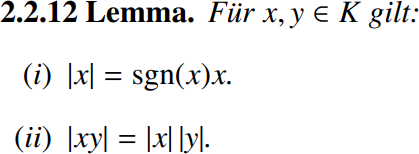
\includegraphics[width = 5 cm]{Kaltenbaeck - Fundament Analysis - Lemma 2-2-12-1.png} \\
      \vspace{0.01 cm}
      \hspace{0.5 cm}
      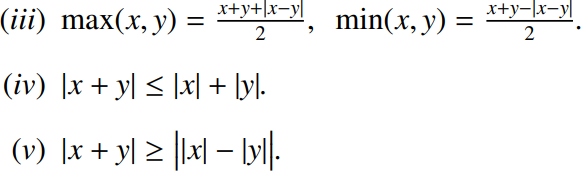
\includegraphics[width = 7 cm]{Kaltenbaeck - Fundament Analysis - Lemma 2-2-12-2.png} \\
      \vspace{0.5 cm}
      \caption{Kaltenbaeck - Fundament Analysis}
      \label{fig:KFAL2.2.12}
    \end{boxedin}
  \end{figure}

  \end{comment}

  Seien $c := 1/2$ und $d := 1$, dann gilt $\ForAlmostAll n \in \N:$

  \begin{multline*}
    c (f(n) + g(n))
    \leq
    \max \Bbraces{f(n), g(n)}
    =
    \frac{f(n) + g(n) + |f(n) - g(n)|}{2} \\
    \leq
    \frac{f(n) + g(n)}{2}
    +
    \frac{f(n) + g(n)}{2}
    =
    d (f(n) + g(n)).
  \end{multline*}

  \item Gegenbeispiel:
  Seien $f \equiv 0$ und $g \equiv 1$, dann gilt $\Forall c, d > 0:$

  \begin{align*}
    c \underbrace{(f(n) + g(n))}_1
    \not \leq
    \underbrace{\min \Bbraces{f(n), g(n)}}_0
    <
    d \underbrace{(f(n) + b(n))}_1.
  \end{align*}

  \begin{align*}
    \implies
    \min \Bbraces{f, g} \not \in \Theta(f + g)
  \end{align*}

  \item Gegenbeispiel:
  Seien $f(n) = n$ und $g(n) = -n$, für $n \in \N$, dann gilt wegen $|f| = |g|$ zwar $f \in \Landau(g)$, aber

  \begin{align*}
    \limsup_{n \to \infty}
    \vbraces
    {
      \frac
      {
        2^{f(n)}
      }{
        2^{g(n)}
      }
    }
    =
    \limsup_{n \to \infty}
    \vbraces
    {
      \frac
      {
        2^{n}
      }{
        2^{-n}
      }
    }
    =
    \limsup_{n \to \infty}
    2^{2n}
    =
    \infty
    \iff
    f \not \in \Landau(g).
  \end{align*}

  Gegenbeispiel:
  Seien $f = \log_2$ und $g = \log_4$, für $n \in \N$, dann gilt wegen $|f| = \log_2{4} |g|$ zwar $f \in \Landau(g)$, aber

  \begin{multline*}
    \limsup_{n  \to \infty}
    \vbraces
    {
      \frac
      {
        2^{f(n)}
      }{
        2^{g(n)}
      }
    }
    =
    \limsup_{n  \to \infty}
    \vbraces
    {
      \frac
      {
        2^{\log_2(n)}
      }{
        2^{\log_4(n)}
      }
    }
    =
    \limsup_{n  \to \infty}
    \vbraces
    {
      \frac
      {
        n
      }{
        2^\frac
        {
          \log_2(n)
        }{
          \log_2(4)
        }
      }
    }
    =
    \limsup_{n  \to \infty}
    \vbraces
    {
      \frac
      {
        n
      }{
        (2^{\log_2(n)})^{1/2}
      }
    } \\
    =
    \limsup_{n  \to \infty}
    \vbraces
    {
      \frac
      {
        n
      }{
        \sqrt{n}
      }
    }
    =
    \limsup_{n  \to \infty}
    \sqrt{n}
    =
    \infty
  \end{multline*}

  \item Gegenbeispiel:
  Sei $f(n) = 1/n$.

  \begin{align*}
    \implies
    \limsup_{n \to \infty}
    \vbraces
    {
      \frac{f(n)}{f(n)^2}
    }
    =
    \limsup_{n \to \infty}
    \vbraces
    {
      \frac{1/n)}{1/n^2}
    }
    =
    \limsup_{n \to \infty} |n|
    =
    \infty
    \iff
    f \not \in \Landau(f^2)
  \end{align*}

  \item Beispiel:

  \begin{align*}
    f(n)
    :=
    \begin{cases}
      0,   & n \in 2 \N, \\
      n^2, & n \in 2 \N - 1,
    \end{cases}
  \end{align*}

  \begin{align*}
    \implies
    \liminf_{n \to \infty}
    \vbraces
    {
      \frac{f(n)}{n}
    }
    & =
    \sup_{n \in \N}
    \inf_{k \geq n}
    \vbraces
    {
      \frac{f(k)}{k}
    }
    =
    0
    \iff
    f(n) \neq \Omega(n), \\
    \limsup_{n \to \infty}
    \vbraces
    {
      \frac{f(n)}{n}
    }
    & =
    \inf_{n \in \N}
    \sup_{k \geq n}
    \vbraces
    {
      \frac{f(k)}{k}
    }
    =
    \infty
    \iff
    f(n) \neq \Landau(n).
  \end{align*}

\end{enumerate}

\end{solution}

% --------------------------------------------------------------------------------

% --------------------------------------------------------------------------------

\begin{exercise}

Zeigen Sie:

\begin{align*}
  f(n) := 2^{2^{\floorbraces{\log_2{(\log_2{n})}}}} = \Landau(n)
\end{align*}

und bestimmen Sie die größte Zahl $c > 0$, sodass

\begin{align*}
  2^{2^{\floorbraces{\log_2{(\log_2{n})}}}} = \Omega(n^c)
\end{align*}

\end{exercise}

% --------------------------------------------------------------------------------

\begin{solution}

\phantom{}

\begin{enumerate}

  \item

  \begin{align*}
    \implies
    \Forall n \in \N:
    2^{2^{\floorbraces{\log_2{(\log_2{n})}}}}
    \leq
    2^{2^{\log_2{(\log_2{n})}}}
    =
    2^{(\log_2{n})}
    =
    n
    =
    \Landau(n)
  \end{align*}

  \item Wir behaupten, dass
  
  \begin{align*}
    1/2 = c := \sup{C},
    \quad
    C := \Bbraces{d > 0: 2^{2^{\floorbraces{\log_2{(\log_2{n})}}}} = \Omega(n^d)}.
  \end{align*}

  \begin{itemize}

    \item
    [\enquote{$\leq$}:]

    \begin{align*}
      & \implies
      \Forall n \in \N:
      2^{2^{\floorbraces{\log_2{(\log_2{n})}}}}
      \geq
      2^{2^{\log_2{(\log_2{n})} - 1}}
      =
      2^{2^{\log_2{(\log_2{(n)})}} / 2}
      =
      (2^{\log_2{n}})^{1/2}
      =
      \sqrt{n}
      =
      \Omega(n^{1/2}) \\
      & \implies
      1/2 \in C
    \end{align*}

    \item
    [\enquote{$\geq$}:]
    Sei $d > 1/2$, dann ist $1/2 - d < 0$.
    Betrachte die Folge $a_n := 2^{2^n} - 1$.

    \begin{align*}
      & \implies
      f(a_n) = 2^{2^{\floorbraces{\log_2{(\log_2{(a_n)})}}}}
      =
      \underbrace
      {
        2^{2^{\floorbraces{\log_2 \pbraces{\log_2 \pbraces{2^{2^n} - 1}}}}}
      }_{
        \stackrel{\text{scharf}}{<}
        2^{2^{\floorbraces{\log_2{\log_2{2^{2^n}}}}}}
        =
        2^{2^n}
      }
      =
      2^{2^{n-1}} \\
      & \implies
      \frac{f(a_n)}{a_n^d}
      =
      \frac{2^{2^{n-1}}}{(2^{2^n} - 1)^d}
      =
      \frac{(2^{2^n})^{1/2}}{(2^{2^n} - 1)^d}
      \leq
      \frac{(2^{2^n})^{1/2}}{(2^{2^n}/2)^d}
      \leq
      2^d \frac{(2^{2^n})^{1/2}}{(2^{2^n})^d}
      =
      2^d (2^{2^n})^{1/2 - d}
      \xrightarrow{n \to \infty}
      0 \\
      & \implies
      \liminf_{n \to \infty}
      \frac{f(n)}{n^d} = 0
      \iff
      f(n) \neq \Omega(n^d) \\
      & \implies
      d \not \in C
    \end{align*}

  \end{itemize}

\end{enumerate}

\end{solution}

% --------------------------------------------------------------------------------

% -------------------------------------------------------------------------------- %

\begin{exercise}[48]

Seien $A = \Bbraces{a_1, \dots, a_n}$ und $B = \Bbraces{b_1, \dots, b_k}$ endliche Mengen.
Sei $P = \Bbraces{p_{i, j} \mid 1 \leq i \leq n, 1 \leq j \leq k}$ eine Menge aussagenlogischer Variablen.
Jede Belegung $b$ von $P$ induziert eine Relation $R_b \subseteq A \times B$ durch $(a_i, b_j) \in R_b$ gdw $b(p_{i, j}) = 1$.
Finden Sie aussagenlogische Formeln $\varphi_1, \varphi_2, \varphi_3, \varphi_4$ so dass:

\begin{enumerate}[label = \arabic*.]
    \item $\hat{b}(\varphi_1) = 1$ gdw $R_b$ ist eine Funktion
    \item $\hat{b}(\varphi_2) = 1$ gdw $R_b$ ist eine injektive Funktion
    \item $\hat{b}(\varphi_3) = 1$ gdw $R_b$ ist eine surjektive Funktion
    \item $\hat{b}(\varphi_4) = 1$ gdw $R_b$ ist eine bijektive Funktion
\end{enumerate}

Für welche $(n, k) \in \N \times \N$ ist $\varphi_2$ unerfüllbar? \\

(
    Anmerkung:
    Die Größe der Formeln hängt von $n$ und $k$ ab.
)

\end{exercise}

% -------------------------------------------------------------------------------- %

\begin{solution}

Nachdem wir Formeln angeben müssen, ist es sicher keine schlechte Idee, die Angabe auch in Formeln aufzuschreiben.

\begin{align*}
  P =
  \begin{Bmatrix}
    p_{11}, & \cdots & p_{1k}, \\
    \vdots  & \ddots & \vdots \\
    p_{n1}, & \cdots & p_{nk}
  \end{Bmatrix},
  \quad
  \begin{matrix}
    A = \Bbraces{a_1, \dots, a_n}, \\
    B = \Bbraces{b_1, \dots, b_k}
  \end{matrix}
\end{align*}

\begin{align*}
  b: p \to \Bbraces{0, 1}
  \rightsquigarrow
  R_b
  =
  \Bbraces
  {
    (a_i, b_j) \in A \times B:
    \:
    \begin{matrix}
      i = 1, \dots, n, \\
      j = 1, \dots, k,
    \end{matrix}
    \quad
    b(p_{ij}) = 1
  }
\end{align*}

\begin{enumerate}[label = \arabic*.]

  \item

  \begin{align*}
    R_b ~\text{Funktion}
    :\iff
    & \Forall a_i \in A:
    \ExistsOnlyOne b_j \in B:
    (a_i, b_j) \in R_b \\
    \iff
    & \Forall a_i \in A:
    \Exists b_j \in B:
    (a_i, b_j) \in R_b
    ~ \land \\
    & \Forall a_i \in A:
    \Forall b_{j_1}, b_{j_2} \in B:
    (a_i, b_{j_1}), (a_i, b_{j_2}) \in R_b
    \implies
    b_{j_1} = b_{j_2} \\
    \iff
    & \Forall a_i \in A:
    \Exists b_j \in B:
    (a_i, b_j) \in R_b
    ~ \land \\
    & \Forall a_i \in A:
    \Forall b_{j_1} \in B:
    (a_i, b_{j_1}) \in R_b
    \implies
    \Forall b_{j_2} \in B \setminus \Bbraces{b_{j_1}}:
    (a_i, b_{j_2}) \not \in R_b
  \end{align*}

  Wir brauchen für unsere Formel also $2$ Bauteile.

  \begin{align*}
    \phi_1
    & :=
    \bigwedge_{i=1}^n \bigvee_{j=1}^kp_{i,j} \\
    \phi_2
    & :=
    \bigwedge_{i=1}^n \bigwedge_{j_1=1}^kp_{i,j_1}
    \to
    \bigwedge_{\substack{j_2=1 \\ j_2\neq j_1}}^{k}\neg p_{i,j_2}
  \end{align*}

  \begin{align*}
    \rightsquigarrow
    \varphi_1 := \phi_1 \land \phi_2
  \end{align*}

  \item Sei $R_b$ eine Funktion.

  \begin{align*}
    R_b ~\text{injektiv}
    :\iff
    & \Forall a_{i_1}, a_{i_2} \in A:
    \Forall b_j \in B:
    (a_{i_1}, b_j), (a_{i_1}, b_j) \in R_b
    \implies
    a_{i_1} = a_{i_2} \\
    \iff
    & \Forall b_j \in B:
    \Forall a_{i_1} \in A:
    (a_{i_1}, b_j) \in R_b
    \implies
    \Forall a_{i_2} \in A \setminus \Bbraces{a_{i_1}}:
    (a_{i_2}, b_j) \not \in R_b
  \end{align*}

  Wir brauchen also noch folgendes, zu $\phi_2$ analoges, Bauteil.

  \begin{align*}
    \phi_3
    :=
    \bigwedge_{j=1}^k \bigwedge_{i_1=1}^np_{i_1,j}
    \to
    \bigwedge_{\substack{i_2=1 \\ i_2\neq i_1}}^{n}\neg p_{i_2,j}
  \end{align*}

  \begin{align*}
    \rightsquigarrow
    \varphi_2
    :=
    \varphi_1 \land \phi_3
  \end{align*}

  % $\varphi_2 = \bigwedge_{i=1}^n \bigvee_{j=1}^k\left(p_{i,j} \land \bigwedge_{l=1,l\neq j}^{k}\neg p_{i,l}\right)
  % \land  \left(\bigwedge_{j=1}^k \bigvee_{i=1}^n\left(p_{i,j} \land \bigwedge_{l=1,l\neq j}^{n}\neg p_{l,j}\right)\right)$

  \item Sei $R_b$ eine Funktion.

  \begin{align*}
    R_b ~\text{surjektiv}
    :\iff
    & \Forall b_j \in B:
    \Exists a_i \in A:
    (a_i, b_j) \in R_b
  \end{align*}

  Wir brauchen also noch folgendes, zu $\phi_1$ analoges, Bauteil.

  \begin{align*}
    \phi_4
    :=
    \bigwedge_{j=1}^k \bigvee_{i=1}^np_{i,j}
  \end{align*}

  \begin{align*}
    \rightsquigarrow
    \varphi_3
    :=
    \varphi_1 \land \phi_4
  \end{align*}

  % $\varphi_3 = \bigwedge_{i=1}^n \bigvee_{j=1}^k\left(p_{i,j} \land \bigwedge_{l=1,l\neq j}^{k}\neg p_{i,l}\right) \land
  % \left(\bigwedge_{j=1}^k \bigvee_{i=1}^np_{i,j}\right)$

  \item Sei $R_b$ eine Funktion.

  \begin{align*}
    R_b ~\text{bijektiv}
    :\iff
    R_b ~\text{injektiv}
    \land
    R_b ~\text{surjektiv}
  \end{align*}

  \begin{align*}
    \rightsquigarrow
    \varphi_4
    :=
    \varphi_2 \land \varphi_3
    =
    \varphi_1 \land \phi_3 \land \phi_4
    =
    \phi_1 \land \phi_2 \land \phi_3 \land \phi_4
  \end{align*}

  % $\varphi_4 = \bigwedge_{i=1}^n \bigvee_{j=1}^k\left(p_{i,j} \land \bigwedge_{l=1,l\neq j}^{k}\neg p_{i,l}\right)
  % \land  \left(\bigwedge_{j=1}^k \bigvee_{i=1}^n\left(p_{i,j} \land \bigwedge_{l=1,l\neq j}^{n}\neg p_{l,j}\right)\right) \land
  % \left(\bigwedge_{j=1}^k \bigvee_{i=1}^np_{i,j}\right)$
\end{enumerate}

Für $k < n$ gibt es keine injektive Funktion von $A$ nach $B$, also ist $\varphi_2$ unerfüllbar, für $k \geq n$ gibt es schon eine, also ist $\varphi_2$ dann erfüllbar.
Das kann man sich auf anschaulich mit einem klassischen Funktions-Diagramm skizzieren:
Zwei getrennte Kreise (Ellipsen), die Punkte beinhalten, die jeweils zwischen den Kreisen verbunden sind.

\end{solution}

% -------------------------------------------------------------------------------- %

\begin{solution}

\phantom{}

\begin{enumerate}[label = \arabic*.]

  \item $\varphi_1 = \bigwedge_{i=1}^n \bigvee_{j=1}^k\left(p_{i,j} \land \bigwedge_{l=1,l\neq j}^{k}\neg p_{i,l}\right)$

  \item $\varphi_2 = \bigwedge_{i=1}^n \bigvee_{j=1}^k\left(p_{i,j} \land \bigwedge_{l=1,l\neq j}^{k}\neg p_{i,l}\right)
  \land  \left(\bigwedge_{j=1}^k \pbraces{\pbraces{\bigvee_{i=1}^n p_{i,j}} \rightarrow \pbraces{\bigvee_{i=1}^n\left(p_{i,j} \land \bigwedge_{l=1,l\neq j}^{n}\neg p_{l,j}\right)}}\right)$

  \item $\varphi_3 = \bigwedge_{i=1}^n \bigvee_{j=1}^k\left(p_{i,j} \land \bigwedge_{l=1,l\neq j}^{k}\neg p_{i,l}\right) \land
  \left(\bigwedge_{j=1}^k \bigvee_{i=1}^np_{i,j}\right)$

  \item $\varphi_4 = \bigwedge_{i=1}^n \bigvee_{j=1}^k\left(p_{i,j} \land \bigwedge_{l=1,l\neq j}^{k}\neg p_{i,l}\right)
  \land  \left(\bigwedge_{j=1}^k \bigvee_{i=1}^n\left(p_{i,j} \land \bigwedge_{l=1,l\neq j}^{n}\neg p_{l,j}\right)\right)$

\end{enumerate}

\end{solution}

% -------------------------------------------------------------------------------- %

\begin{exercise}

Gegeben ist die Funktion $F: \R \to \R:$

\begin{align*}
  F(x) =
  \begin{cases}
    0   & \text{wenn} \enspace x < 0, \\
    1   & \text{wenn} \enspace 0 \leq x < 1, \\
    x^2 & \text{wenn} \enspace 1 \leq x < 2, \\
    5   & \text{wenn} \enspace x \geq 2.
  \end{cases}
\end{align*}

\begin{itemize}
  \item[(a)] Zeigen Sie, dass $F$ eine Verteilungsfunktion ist.
  \item[(b)] Bestimmen Sie $\mu_F(]0, 1[)$, $\mu_F([0, 2])$, $\mu_F(\Q)$.
  \item[(c)] Bestimmen Sie $\Int{e^x}{\mu_F(x)}$.
\end{itemize}

\end{exercise}

--------------------------------------------------------------------------------

\begin{solution}

(a)

\begin{itemize}

  \item \Quote{Rechtsstetigkeit}: $F$ ist stückweise stetig und $\Forall x = 0, 1, 2: F \text{ist rechtsstetig bei} \enspace x$.

  \item \Quote{Steigende Monotonie}: $F$ ist stückweise monoton steigend und $\Forall x = 0, 1, 2: F(x - 0) \leq F(x)$.

\end{itemize}

(b)

\begin{itemize}

  \item $\mu_F(]0, 1[) =$
  \begin{align*}
    \mu_F \pbraces{\bigcup_{n \in \N} \left ] 0, 1 - \frac{1}{n} \right ]}
    =
    \lim_{n \in \N} \mu_F \pbraces{\left ] 0, 1 - \frac{1}{n} \right ]}
    =
    \lim_{n \in \N} F \pbraces{1 - \frac{1}{n}} - F(0)
    = 1 - 1 = 0
  \end{align*}

  \item $\mu_F([0, 2]) =$
  \begin{align*}
    \mu_F \pbraces{\bigcap_{n \in \N} \left ] 0 - \frac{1}{n}, 2 \right ]}
    =
    \lim_{n \in \N} \mu_F \pbraces{\left ] 0 - \frac{1}{n}, 2 \right ]}
    =
    \lim_{n \in \N} F(2) - F \pbraces{0 - \frac{1}{n}}
    =
    5 - 0 = 5
  \end{align*}

  \item $\mu_F(\Q) =$
  \begin{align*}
    \mu_F \pbraces{\sum_{q \in \Q} \Bbraces{q}}
    & =
    \sum_{q \in \Q} \mu_F \pbraces
    {\bigcap_{n \in \N} \left ] q - \frac{1}{n}, q \right ]} \\
    & =
    \sum_{q \in \Q} \lim_{n \in \N} \mu_F \pbraces
    {\left ] q - \frac{1}{n}, q \right ]} \\
    & =
    \sum_{q \in \Q} F(q - 0) - F(q) \\
    & =
    \sum_{x = 0, 1, 2} (F(x) - F(x - 0)) \\
    & =
    (1 - 0) + (1 - 1) + (5 - 4) = 2
  \end{align*}

\end{itemize}

(c) Seien $f = \exp$ und $a_1, \ldots, a_n$ die Sprünge von $F$, sowie $a_0 = - \infty$ und $a_{n+1} = \infty$.

\begin{align*}
  \Int{f}{\mu_F}
  =
  \sum_{i=1}^{n+1} \Int[a_{i-1}][a_i]{f(x) F^\prime(x)}{x} +
  \sum_{i=1}^n f(a_i) (F(a_i) - F(a_i - 0))
\end{align*}

Also ...

\begin{align*}
  \Int{e^x}{\mu_F(x)}
  & =
  \underbrace{\Int[-\infty][0]{e^x 0}{x}}_0
  +
  \underbrace{\Int[0][1]{e^x 0}{x}}_0
  +
  \Int[1][2]{e^x 2x}{x}
  +
  \underbrace{\Int[2][\infty]{e^x 0}{x}}_0 \\
  & +
  e^0 \underbrace{(F(0) - F(0 - 0))}_{= 1-0 = 1}
  +
  e^1 \underbrace{(F(1) - F(1 - 0))}_{= 1-1 = 0}
  +
  e^2 \underbrace{(F(2) - F(2 - 0))}_{= 5-4 = 1} \\
  & =
  e^x 2x |_1^2 - 2 \Int[1][2]{e^x}{x} + 1 + e^2 \\
  & =
  (4e^2 - 2e) - 2 (e^2 - e) + 1 + e^2
  =
  1 + 3e^2
\end{align*}

\end{solution}

% --------------------------------------------------------------------------------

\begin{exercise}[Exercise 3.8]

Suppose $\gamma = 0.5$ and the following sequence of rewards is received $R_1 = -1$, $R_2 = 2$, $R_3 = 6$, $R_4 = 3$, and $R_5 = 2$, with $T = 5$.
What are $G_0, G_1 , \dots, G_5$?
Hint:
Work backwards.    

\end{exercise}

% --------------------------------------------------------------------------------

\begin{solution}

ToDo!

\end{solution}

% --------------------------------------------------------------------------------

% --------------------------------------------------------------------------------

\begin{exercise}[36]

ToDo!

\end{exercise}

% --------------------------------------------------------------------------------

\begin{solution}

Außer Konkurrenz!

\end{solution}

% --------------------------------------------------------------------------------

% --------------------------------------------------------------------------------

\begin{exercise}

Berechnen Sie

\begin{align*}
    \Int[0][\infty]
    {
        \frac
        {
            \arctan(x)
        }{
            (1 + x^2) x
        }
    }{x}
\end{align*}

indem Sie für $\lambda > -1$ die Funktion

\begin{align*}
    F(\lambda)
    :=
    \Int[0][\infty]
    {
        \frac
        {
            \arctan(\lambda x)
        }{
            (1 + x^2) x
        }
    }{x}
\end{align*}

differenzieren.

\end{exercise}

% --------------------------------------------------------------------------------

\begin{solution}

\phantom{}

\begin{enumerate}[label = \arabic*.]

    \item Versuch (naiv):
    
    Wir betrachten die Folgende Familie von Funktionen.

    \begin{align*}
        f_\lambda(x)
        :=
        \frac
        {
            \arctan(\lambda x)
        }{
            (1 + x^2) x
        },
        \quad
        x \in (0, 1),
        \quad
        \lambda > -1
    \end{align*}

    Dafür finden wir eine, von $\lambda$, unabhängige Majorante.

    \begin{align*}
        \abs
        {
            \pderivative[][f_\lambda(x)]{\lambda}
        }
        =
        \abs
        {
            \pderivative{\lambda}
            \frac
            {
                \arctan(\lambda x)
            }{
                (1 + x^2) x
            }    
        }
        =
        \abs
        {
            \frac{x}
            {
                1 + (\lambda x)^2
            }    
            \frac{1}
            {
                (1 + x^2) x
            }    
        }
        =
        \underbrace
        {
            \frac{1}
            {
                1 + (\lambda x)^2
            }        
        }_{
            \leq 1
        }
        \frac{1}
        {
            1 + x^2
        }    
        \leq
        \frac{1}
        {
            1 + x^2
        }
        =:
        g(x)
    \end{align*}

    Die Majorante $g$ ist auf $(0, \infty)$ auch integrierbar.

    \begin{align*}
        \Int[0][\infty]{g(x)}{x}
        =
        \Int[0][\infty]
        {
            \frac{1}
            {
                1 + x^2
            }    
        }{x}
        =
        \arctan x \Big |_{x=0}^\infty
        =
        \frac{\pi}{2}
        <
        \infty
    \end{align*}

    Wir können daher die folgende Vertauschung des Differenzialoperators mit dem Integral durchführen.

    \begin{align*}
        \derivative{\lambda}
        F(\lambda)
        =
        \derivative{\lambda}
        \Int[0][\infty]{f_\lambda(x)}{x}
        =
        \Int[0][\infty]
        {
            \pderivative{\lambda}
            f_\lambda(x)
        }{x}
        =
        \Int[0][\infty]
        {
            \frac{1}
            {
                1 + (\lambda x)^2
            }    
            \frac{1}
            {
                1 + x^2
            }    
        }{x}
        \stackrel
        {
            \mathrm{Integralrechner}
        }{=}
        \frac{\pi}{2 (\lambda + 1)}
    \end{align*}

    Wir benutzen nun den Hauptsatz der Differezial- und Integral-Rechnung.

    \begin{align*}
        \Int[0][\infty]
        {
            \frac
            {
                \arctan(x)
            }{
                (1 + x^2) x
            }
        }{x}
        =
        F(1) - \underbrace{F(0)}_0
        \stackrel
        {
            \mathrm{HS}
        }{=}
        \Int[0][1]
        {
            \derivative{\lambda}
            F(\lambda)
        }{\lambda}
        =
        \frac{\pi}{2}
        \Int[0][1]
        {
            \frac{1}{\lambda + 1}
        }{\lambda}
        =
        \frac{\pi}{2}
        \ln(\lambda + 1) \Big |_{\lambda = 0}^1
        =
        \frac{\pi}{2}
        \ln 2
    \end{align*}

    \item Versuch (rigoros):
    
    Wir wollen nun noch zeigen, dass $F$ wohldefiniert, d.h. endlich, ist.
    Weil der $\arctan$ eine ungerade Funktion ist, d.h. das $-$ rutscht durch, betrachten wir o.B.d.A. bloß $\lambda \geq 0$.
    Wir setzen den Integranden $f_\lambda$ von $F$ stetig auf $0$ fort.

    \begin{align*}
        f_\lambda(0)
        :=
        \lim_{x \to 0}
        f_\lambda(x)
        \stackrel
        {
            \mathrm{L'Hospital}
        }{=}
        \lim_{x \to 0}
        \frac
        {
            \frac{1}{1 + x^2}
            \lambda
        }{
            1 + 3 x^2
        }
        =
        \lambda
    \end{align*}

    Wir wollen nun zeigen, dass $f_\lambda(x)$ monoton fallend in $x$ ist.

    \begin{align*}
        & \iff
        \pderivative{x}
        f_\lambda(x)
        \stackrel
        {
            \mathrm{Ableitungsrechner}
        }{=}
        \frac{\lambda}
        {
            (\lambda^2 x^2 + 1)
            (x^3 + x)
        }
        -
        \frac
        {
            (3 x^2 + 1)
            \arctan(\lambda x)
        }{
            (x^3 + x)^2
        }
        \leq 0 \\
        & \iff
        \frac{\lambda}
        {
            (\lambda^2 x^2 + 1)
            (x^3 + x)
        }
        \leq
        \frac
        {
            (3 x^2 + 1)
            \arctan(\lambda x)
        }{
            (x^3 + x)^2
        } \\
        & \impliedby
        \lambda (x^3 + x)
        \stackrel{!}{\leq}
        (\lambda^2 x^2 + 1) (3 x^2 + 1)
        \stackrel{!}{\leq}
        (\lambda^2 x^2 + 1) (3 x^2 + 1) \arctan(\lambda x) \\
    \end{align*}

    Die linke Seite ist ein Polynom $3$-ten und die Mitte ein Polynom $4$-ten Grades in $x$.
    Daher glit die $1$-te Ungleichung ab einem gewissen $x_{\lambda, 1} \in \N$.
    Weil $\lambda > 0$, ist $\arctan(\lambda x)$ in $x$ monoton steigend gegen $\frac{\pi}{2}$.

    \begin{align*}
        \implies
        \Exists x_{\lambda, 1} \in \N:
        \Forall x \geq x_{\lambda, 1}:
        \arctan(\lambda x) \geq 1
    \end{align*}

    Die $1$-te und $2$-te Ungleichung gelten also beide ab $x_\lambda := \max(x_{\lambda, 1}, x_{\lambda, 2})$.
    $f_\lambda$ ist also in $[x_\lambda, \infty)$ monoton fallend.

    \begin{align*}
        F(\lambda)
        :=
        \Int[0][\infty]
        {
            f_\lambda(x)
        }{x}
        =
        \Int[0][x_\lambda]
        {
            f_\lambda(x)
        }{x}
        +
        \Int[x_\lambda][\infty]
        {
            f_\lambda(x)
        }{x}
        \stackrel{!}{<}
        \infty
    \end{align*}

    Das $1$-te $\int$ ist, als $\int$ einer stetigen Funktion auf dem Kompaktum $[0, x_\lambda]$, endlich;
    das $2$-te untersuchen wir jetzt-dann.

    Zuerst beweisen wir noch, dass

    \begin{align*}
        \Forall x \in [0, \infty): \arctan x \leq x.
    \end{align*}

    Für $x = 0$ gilt sogar Gleichheit.
    Die Ungleichung geht für $x > 0$ nicht verlohren, weil wenn sie für $x = 0$ stimmt, dann ist

    \begin{align*}
        x - \arctan x \geq 0
        & \iff
        x - \arctan x ~\text{monoton steigend}~ \\
        & \iff
        \derivative{x}
        (x - \arctan x)
        =
        1 - \frac{1}{1 + x^2}
        \geq
        0 \\
        & \iff
        1 + x^2 \geq 1.
    \end{align*}

    Wir kommen nun aber endlich zu unseren finalen Abschätzung.

    \begin{align*}
        \Int[x_\lambda][\infty]
        {
            \frac
            {
                \arctan(\lambda x)
            }{
                (1 + x^2) x
            }
        }{x}
        \leq
        \sum_{n = x_\lambda}^\infty
        f_\lambda(n)
        =
        \sum_{n = x_\lambda}^\infty
        \frac
        {
            \arctan(\lambda n)
        }{
            (1 + n^2) n
        }
        \leq
        \sum_{n = x_\lambda}^\infty
        \frac{n}
        {
            (1 + n^2) n
        }
        \leq
        2
        \sum_{n = x_\lambda}^\infty
        \frac{1}{n^2}
        <
        \infty
    \end{align*}

\end{enumerate}

\end{solution}

% --------------------------------------------------------------------------------

% --------------------------------------------------------------------------------

\begin{exercise}

Sei $(M, \metric)$ ein metrischer Raum.
Dann ist $M \times M$ mit der Maximumsmetrik $\metric_m((x_1, x_2), (y_1, y_2)) := \max(\metric(x_1, y_1), \metric(x_2, y_2))$ ein metrischer Raum und für eine Vervollständigung $(\tilde M, \tilde \metric)$ von $M$ ist $\tilde M \times \tilde M$ mit der Maximumsmetrik eine Vervollständigung von $M \times M$.

\end{exercise}

% --------------------------------------------------------------------------------

\begin{solution}

\phantom{}

\begin{enumerate}[label = \arabic*.]

    \item Teil:
    
    Wir zeigen, dass $\metric_{\max} := \metric_m$ eine Metrik ist.
    Dazu überprüfen (bzw. behaupten) wir $\Forall x, y, z \in M^2$ die folgenden 4 Eigenschaften.
    
    \begin{enumerate}[label = \arabic*.]

        \item Eigenschaft (Nicht-Negativität):
        
        \begin{align*}
            \text{d.h.}~
            \metric_{\max}(x, y) \geq 0
        \end{align*}

        \item Eigenschaft (Definitheit):
        
        \begin{align*}
            \text{d.h.}~
            \metric_{\max}(x, y) = 0 \iff x = y
        \end{align*}

        \item Eigenschaft (Symmetrie):
        
        \begin{align*}
            \text{d.h.}~
            \metric_{\max}(x, y) = \metric_{\max}(y, x)
        \end{align*}

        \item Eigenschaft (Dreiecksungleichung):
        
        \begin{align*}
            \text{d.h.}~
            \metric_{\max}(x, y)
            +
            \metric_{\max}(y, z)
            \leq
            \metric_{\max}(x, z)
        \end{align*}

    \end{enumerate}

    \item Teil:
    
    \includegraphicsboxed{Ana1&2/Ana1&2 - 6.7.1 Definition.png}

    Wir zeigen also, dass folgender metrischer Raum vollständig ist und es eine passende Isometrie gibt.
    Laut dem 1. Teil ist er ja bereits ein metrischer Raum, weil $(\tilde M, \tilde \metric)$ einer ist.

    \begin{align*}
        (\tilde M^2, \tilde \metric_{\max}),
        \quad
        \metric_{\max}(x, y)
        :=
        \max
        (
            \tilde \metric(x_1, y_1),
            \tilde \metric(x_2, y_2)
        )
    \end{align*}

    \begin{enumerate}[label = 2.\arabic*.]

        \item Teil (Vollständigkeit):
        
        Sei dazu $(x_n)_{n \in \N} \in (\tilde M^2)^\N$ eine Cauchy-Folge bzgl. $\tilde \metric_{\max}$, d.h.

        \begin{align*}
            \Forall \varepsilon > 0:
            \Exists N \in \N:
            \Forall n, m \geq N:
            \varepsilon
            >
            \tilde \metric_{\max}(x_n, x_m)
            =
            \max
            (
                \tilde \metric(x_{n, 1}, x_{m, 1}),
                \tilde \metric(x_{n, 2}, x_{m, 2})
            ).
        \end{align*}

        Offenbar sind dann $(x_{n, 1})_{n \in \N}, (x_{n, 2})_{n \in \N} \in (\tilde M^2)^\N$ Cauchy-Folgen bzgl. $\tilde \metric$.
        Weil $(\tilde M, \tilde \metric)$ ja vollständig ist, konvergieren die gegen Grenzwerte $x_1 \in \tilde M$ bzw. $x_2 \in \tilde M$.

        Unseren Grenzwert-Kandidat für $(x_n)_{n \in \N} \in (\tilde M^2)^\N$ setzen wir also gleich $x := (x_1, x_2)$.
        Dieser ist nicht nur ein Kandidat, weil

        \begin{align*}
            \tilde \metric_{\max}(x_n, x)
            =
            \max
            (
                \tilde \metric(x_{n, 1}, x_1),
                \tilde \metric(x_{n, 2}, x_2)
            )
            \xrightarrow{n \to \infty}
            0.
        \end{align*}

        \item Teil (Isometrie):
        
        Weil $(\tilde M, \tilde \metric)$ eine Vervollständigung von $(M, \metric)$ ist,

        \begin{align*}
            \Exists \iota:
            (M, \metric) \to (\tilde M, \tilde \metric) ~\text{Isometrie}:
            \overline{\iota(M)} = \tilde M.
        \end{align*}

        Daraus können wir einen Kandidaten für $(\tilde M^2, \tilde \metric_{\max})$ basteln.

        \begin{align*}
            \iota^2:
            (M^2, \metric_{\max})
            \to
            (\tilde M^2, \tilde \metric_{\max}):
            (x_1, x_2)
            \mapsto
            (
                \iota(x_1),
                \iota(x_2)
            )
        \end{align*}

        $\iota^2$ ist tatsächlich isometrisch, weil $\iota$ eine ist, also $\Forall x, y \in M^2:$

        \begin{align*}
            \metric_{\max}(x, y)
            =
            \max
            (
                \metric(x_1, y_1),
                \metric(x_2, y_2)
            )
            =
            \max
            (
                \tilde \metric(\iota(x_1), \iota(y_1)),
                \tilde \metric(\iota(x_2), \iota(y_2))
            )
            =
            \tilde \metric_{\max}(\iota^2(x), \iota^2(y)).
        \end{align*}

        Für die Dichtheit des Bildes von $\iota^2$, d.h. $\overline{\iota^2(M^2)} = \tilde M^2$, sind 2 Inklusionen zu zeigen.

        \begin{enumerate}[label = \arabic*.]

            \item Inklusion (\enquote{$\subseteq$}):

            \item Inklusion (\enquote{$\supseteq$}):
            
            Sei $y \in \tilde M^2$, also dessen Komponenten $y_1, y_2 \in \tilde M$.
            Weil ja $\overline{\iota(M)} = \tilde M$, finden wir $2$ Folgen aus $\iota(M)$, die gegen $y_1$ bzw. $y_2$ konvergieren, d.h. $\Exists (y_{1, n})_{n \in \N}, (y_{2, n})_{n \in \N} \in \iota(M):$

            \begin{align*}
                y_{1, n} \xrightarrow[n \to \infty]{\tilde \metric} y_1,
                \quad
                y_{2, n} \xrightarrow[n \to \infty]{\tilde \metric} y_2.
            \end{align*}

            Daraus können wir den Kandidaten $(y_{1, n}, y_{2, n})_{n \in \N}$ basteln.
            Diese Folge muss nun aus $\iota^2(M^2)$ sein und gegen $y$ konvergieren.
            
            Laut Definition des Bildes $\iota(M)$, $\Exists (x_{1, n})_{n \in \N}, (x_{2, n})_{n \in \N} \in M^\N: \Forall n \in \N:$

            \begin{align*}
                & \iota(x_{1, n}) = y_{1, n},
                \quad
                \iota(x_{2, n}) = y_{2, n} \\
                \implies
                & (x_{1, n}, x_{2, n}) \in M^2 \\
                \implies
                & \iota^2(M^2)
                \ni
                \iota^2((x_{1, n}, x_{2, n}))
                =
                (
                    \iota(x_{1, n}),
                    \iota(x_{2, n})
                )
                =
                (y_{1, n}, y_{2, n})
                \xrightarrow[n \to \infty]{\tilde \metric_{\max}}
                (y_1, y_2)
                =
                y.
            \end{align*}

        \end{enumerate}

    \end{enumerate}

\end{enumerate}

\end{solution}

% --------------------------------------------------------------------------------

\begin{exercise}
Figure \ref{fig:2.21} (below) gives the optimal value of the best state of the gridworld as $24.4$, to one decimal place.
Use your knowledge of the optimal policy and \eqref{eq:2.15} to express this value symbolically, and then to compute it to three decimal places.

\begin{figure}[H]
    \centering
    \subfloat[Gridworld]
    {
        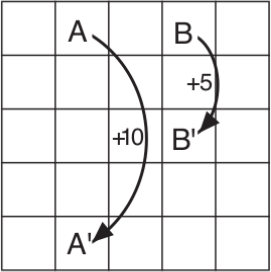
\includegraphics[width = 0.2 \textwidth]{2.21.1.png}
    }
    \hspace{1cm}
    \subfloat[$v_\ast$]
    {
        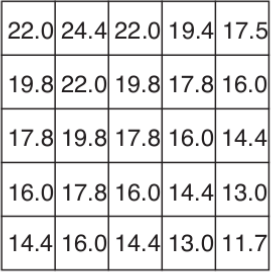
\includegraphics[width = 0.2 \textwidth]{2.21.2.png}
    }
    \hspace{1cm}
    \subfloat[$\pi_\ast$]
    {
        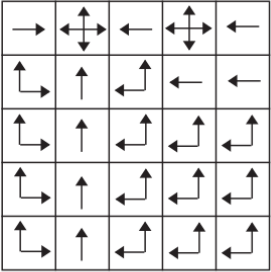
\includegraphics[width = 0.2 \textwidth]{2.21.3.png}
    }
    \hspace{0mm}
    \caption
    {
        Optimal solutions to the gridworld example.
    }
    \label{fig:2.21}
    \end{figure}
\end{exercise}

\begin{solution}
  Once we are in the best state $A$ and follow the optimal policy, we get a reward of $10$ for moving out of the state and then move up again, getting no reward for $4$ steps until we are in state $A$ again. With this we compute

  \begin{align*}
    v_*(A)
    &=
    \E_{\pi_*}\bigg[\sum_{k=0}^\infty \gamma^k R_{t+k+1}\mid S_t = A\bigg]
    =
    \sum_{k=0}^\infty \gamma^k \E_{\pi_*}\bigg[R_{t+k+1}\mid S_t = A\bigg] \\
    &=
    \sum_{k=0}^\infty \gamma^k \1_{\{k = 0 \mod 5\}} \cdot 10
    =
    10 \cdot \sum_{k=0}^\infty \big(\gamma^5\big)^k
    =
    \frac{10}{1-(0.9)^5}
    \approx
    24,4194
  \end{align*}
\end{solution}

% -------------------------------------------------------------------------------- %

\begin{exercise}

Zeigen Sie, dass für $f, g \in L^1(\R^n)$ $\supp(f \ast g)$ keine Teilmenge von $\supp(f) + \supp(g)$ sein muss.

\end{exercise}

% -------------------------------------------------------------------------------- %

\begin{solution}

Wir erinnern uns zunächst an folgende Definitionen.

\begin{align*}
    \supp f
    :=
    \overline
    {
        \Bbraces
        {
            x \in \R^n:
            f(x) \neq 0
        }
    },
    \quad
    A + B
    :=
    \Bbraces
    {
        a + b:
        a \in A,
        b \in B
    },
    \quad
    A, B \subseteq \R^n
\end{align*}

Die folgenden Mengen $X, Y$ sind zwar abgeschlossen, ihre Summe $X + Y$ aber nicht.

\begin{gather*}
    X := \Bbraces{x \in \R^2: x_1 > 0, x_1 x_2 \geq 1} \subset \R^+ \times \R^+,
    \quad
    Y := \Bbraces{x \in \R^2: y_1 > 0, y_1 y_2 \leq -1} \subset \R^+ \times \R^- \\
    \implies
    X + Y = \R^+ \times \R
\end{gather*}

Damit konstruieren wir unsere Kandidaten.

\begin{align*}
    f(x)
    :=
    e^{-(x_1 + x_2)} \1_X(x),
    \quad
    x \in \R^2,
    \quad
    g(y)
    :=
    e^{-(y_1 - y_2)} \1_Y(y),
    \quad
    y \in \R^2
\end{align*}

Diese sind in der Tat integrierbar, d.h. $f, g \in L^1(\R^2)$.

\begin{align*}
    \norm[L^1(\R^2)]{f}
    & =
    \Int[\R^2]{|f|}{\lambda^2}
    \leq
    \underbrace
    {
        \pbraces
        {
            \Int[0][\infty]{e^{-x_1}}{x_1}
        }
    }_1
    \underbrace
    {
        \pbraces
        {
            \Int[0][\infty]{e^{-x_2}}{x_2}
        }
    }_1
    <
    \infty, \\
    \norm[L^1(\R^2)]{g}
    & =
    \Int[\R^2]{|g|}{\lambda^2}
    \leq
    \underbrace
    {
        \pbraces
        {
            \Int[0][\infty]{e^{y_1}}{y_1}
        }
    }_1
    \underbrace
    {
        \pbraces
        {
            \Int[-\infty][0]{e^{-y_2}}{y_2}
        }    
    }_1
    <
    \infty
\end{align*}

Wir berechnen deren Faltung an der Stelle $\pbraces{\frac{1}{n}, 0}$ für $n \in \N$.

\begin{multline*}
    (f \ast g) \pbraces{\frac{1}{n}, 0}
    =
    \Int[\R^2]{f \pbraces{\frac{1}{n} - y_1} g(y)}{\lambda^2(y)} \\
    =
    \Int[\R^2]
    {
        e^{y_1 + y_2 - \frac{1}{n}}
        \1_X \pbraces{\frac{1}{n} - y_1, -y_2}
        e^{-(y_1 - y_2)}
        \1_Y(y)
    }{\lambda^2(y)}
    =
    \cdots
\end{multline*}

\begin{align*}
    y \in Y
    \iff
    \begin{cases}
        y_1 > 0, \\
        y_1 y_2 \leq -1 \iff y_2 \leq -\frac{1}{y_1}
    \end{cases}
\end{align*}

\begin{multline*}
    \implies
    \cdots
    =
    \Int[0][\infty]
    {
        \Int[-\infty][-\frac{1}{y_1}]
        {
            e^{2 y_2 - \frac{1}{n}}
            \1_X \pbraces{\frac{1}{n} - y_1, y_2}
        }{y_2}
    }{y_1} \\
    =
    \Int[0][\infty]
    {
        \Int[\frac{1}{y_1}][\infty]
        {
            e^{-(2 y_2 + \frac{1}{n})}
            \1_X \pbraces{\frac{1}{n} - y_1, y_2}
        }{y_2}
    }{y_1}
    =
    \cdots
\end{multline*}

\begin{align*}
    \pbraces{\frac{1}{n} - y_1, y_2} \in X
    \iff
    \begin{cases}
        \frac{1}{n} - y_1 > 0 \iff \frac{1}{n} > y_1 \\
        \pbraces{\frac{1}{n} - y_1} y_2 \geq 1 \iff y_2 \geq \frac{n}{1 - n y_1}
    \end{cases}
\end{align*}

\begin{align*}
    \implies
    \cdots
    =
    \Int[0][\frac{1}{n}]
    {
        \Int[\frac{n}{1 - n y_1}][\infty]
        {
            e^{-(2 y_2 + \frac{1}{n})}
        }{y_2}
    }{y_1}
    >
    0
\end{align*}

Damit ist also die ganze Folge $\pbraces{\frac{1}{n}, 0}_{n \in \N} \subset \supp(f \ast g)$.
Weil der $\supp$ abgeschlossen ist, liegt auch $0 \in \supp(f \ast g)$.

$X$ und $Y$ sind, wie gesagt, abgeschlossen.

\begin{align*}
    \implies
    \supp f \subset X,
    \quad
    \supp g \subset Y
    \implies
    \supp f + \supp g \subset X + Y = \R^+ \times \R
\end{align*}

$0$ liegt allerdings in keiner Mengen-Summe.

\begin{align*}
    0 \not \in \R^+ \times \R = X + Y
    \implies
    0
    \begin{cases}
        \not \in \supp f + \supp g, \\
        \in \supp(f \ast g)
    \end{cases}
    \implies
    \supp f + \supp g
    \not \subset
    \supp(f \ast g)
\end{align*}

\end{solution}

% -------------------------------------------------------------------------------- %

% -------------------------------------------------------------------------------- %

\begin{exercise}

Berechnen SIe die Faltung $f \ast g$ der Funktion

\begin{align*}
    f(x)
    & =
    \begin{cases}
        e^{-\alpha x} & x > 0 \\
        0             & \text{sonst}
    \end{cases} \\
    g(x)
    & =
    \begin{cases}
        e^{-\beta x} & x > 0 \\
        0            & \text{sonst}
    \end{cases}
\end{align*}

für $\alpha, \beta > 0$.

\end{exercise}

% -------------------------------------------------------------------------------- %

\begin{solution}

\phantom{}

\begin{align*}
    (f \ast g)(x)
    =
    \Int[\R]{f(x - y) g(y)}{\lambda(y)}
    =
    \cdots
\end{align*}

\begin{align*}
    f(x - y) \neq 0
    & \iff
    x - y > 0
    \iff
    x > y \\
    g(y) \neq 0
    & \iff
    y > 0 \\
    & \implies
    \Bbraces{y \in \R: f(x - y) g(y) \neq 0}
    =
    \Bbraces{y \in \R: x > y > 0}
    =
    (0, x)
\end{align*}

\begin{multline*}
    \implies
    \cdots
    =
    \1_{\R^+}(x)
    \Int[0][x]
    {
        e^{-\alpha (x - y)}
        e^{-\beta y}
    }{y}
    =
    \1_{\R^+}(x)
    e^{-\alpha x}
    \Int[0][x]
    {
        e^{(\alpha - \beta) y}
    }{y} \\
    =
    \1_{\R^+}(x)
    e^{-\alpha x}
    \begin{cases}
        x,
        & \alpha = \beta, \\
        \frac
        {
            e^{(\alpha - \beta) x - 1}
        }{
            \alpha - \beta
        },
        & \text{sonst}
    \end{cases}
\end{multline*}

\end{solution}

% -------------------------------------------------------------------------------- %

% --------------------------------------------------------------------------------

\begin{exercise}[Exercise 3.18]

The value of a state depends on the values of the actions possible in that state and on how likely each action is to be taken under the current policy.
We can think of this in terms of a small backup diagram rooted at the state and considering each possible action:

\begin{figure}[H]
    \centering
    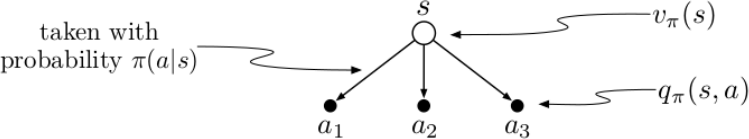
\includegraphics[width = 0.5 \textwidth]{2.18.png}
    \caption{}
    \label{fig:2.18}
\end{figure}

Give the equation corresponding to this intuition and diagram for the value at the root node, $v_\pi(s)$, in terms of the value at the expected leaf node, $q_\pi(s, a)$, given $S_t = s$.
This equation should include an expectation conditioned on following the policy, $\pi$.
Then give a second equation in which the expected value is written out explicitly in terms of $\pi(a \mid s)$ such that no expected value notation appears in the equation.

\end{exercise}

% --------------------------------------------------------------------------------

\begin{solution}

\begin{align*}
    v_\pi(s)
    \doteq
    \E_\pi[G_t \mid S_t = s]
    =
    \sum_a
        \pi(a \mid s)
        \E_\pi[G_t \mid S_t = s, A_t = a]
    =
    \sum_a
        \pi(a \mid s)
        q_\pi(a, s)
\end{align*}

\end{solution}

% --------------------------------------------------------------------------------

% --------------------------------------------------------------------------------

\begin{exercise}[Exercise 3.19]

The value of an action, $q_\pi(s, a)$, depends on the expected next reward and the expected sum of the remaining rewards.
Again we can think of this in terms of a small backup diagram, this one rooted at an action (state-action pair) and branching to the possible next states:

\begin{figure}[H]
    \centering
    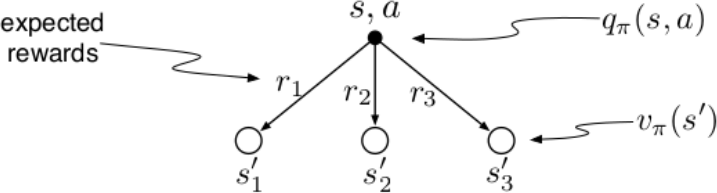
\includegraphics[width = 0.5 \textwidth]{2.19.png}
    \caption{}
    \label{fig:2.19}
\end{figure}

Give the equation corresponding to this intuition and diagram for the action value, $q_\pi(s, a)$, in terms of the expected next reward, $R_{t+1}$ , and the expected next state value, $v_\pi(S_{t+1})$, given that $S_t = s$ and $A_t = a$.
This equation should include an expectation but not one conditioned on following the policy.
Then give a second equation, writing out the expected value explicitly in terms of $p(s_0, r \mid s, a)$ defined by \eqref{eq:2.13}, such that no expected value notation appears in the equation.

\end{exercise}

% --------------------------------------------------------------------------------

\begin{solution}

\begin{align*}
    q_\pi(s, a)
    & =
    \E_\pi[G_t \mid S_t = s, A_t = a] \\
    & =
    \E_\pi[R_{t+1} + \gamma G_{t+1} \mid S_t = s, A_t = a] \\
    & =
    \sum_{s^\prime, r}
        p(s^\prime, r \mid s, a)
        \E_\pi[R_{t+1} + \gamma G_{t+1} \mid S_t = s, A_t = a, S_{t+1} = s^\prime, R_{t+1} = r] \\
    & =
    \sum_{s^\prime, r}
        p(s^\prime, r \mid s, a)
        E_\pi[r + \gamma G_{t+1} \mid S_t = s, A_t = a, S_{t+1} = s^\prime] \\
    & =
    \sum_{s^\prime, r}
        p(s^\prime, r \mid s, a)
        \pbraces
        {
            r + \gamma \E_\pi[G_{t+1} \mid S_t = s, A_t = a, S_{t+1} = s^\prime]
        } \\
    & =
    \sum_{s^\prime, r}
        p(s^\prime, r \mid s, a)
        (r + \gamma v_\pi(s^\prime)) \\
    & =
    \sum_{s^\prime}
        \pbraces
        {
            p(s^\prime \mid s, a)
            \sum_r
                r
                \frac
                {
                    p(s^\prime, r \mid s, a)
                }{
                    p(s^\prime \mid s, a)
                }
            +
            \gamma v_\pi(s^\prime)
            \sum_r
                p(s^\prime, r \mid s, a)
        } \\
    & =
    \sum_{s^\prime}
        \pbraces
        {
            p(s^\prime \mid s, a)
            r(s, a, s^\prime)
            +
            \gamma v_\pi(s^\prime)
            p(s^\prime \mid s, a)
        } \\
    & =
    \sum_{s^\prime}
        p(s^\prime \mid s, a)
        \pbraces
        {
            r(s, a, s^\prime)
            +
            \gamma v_\pi(s^\prime)
        } \\
    & =
    \E[R_{t+1} + \gamma v_\pi(S_{t+1}) \mid S_t = s, A_t = a]
\end{align*}

\end{solution}

% --------------------------------------------------------------------------------

% --------------------------------------------------------------------------------

\begin{exercise}[Exercise 3.22]

Consider the continuing MDP shown below.
The only decision to be made is that in the top state, where two actions are available, \textbf{left} and \textbf{right}.
The numbers show the rewards that are received deterministically after each action.
There are exactly two deterministic policies, $\pi_\textbf{left}$ and $\pi_\textbf{right}$.
What policy is optimal if $\gamma = 0$?
If $\gamma = 0.9$?
If $\gamma = 0.5$?

\begin{figure}[H]
    \centering
    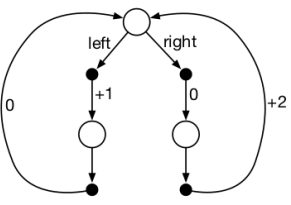
\includegraphics[width = 0.25 \textwidth]{2.20.png}
    \caption{}
    \label{fig:2.20}
\end{figure}

\end{exercise}

% --------------------------------------------------------------------------------

\begin{solution}

When using the policies $\pi_\text{left}$ or $\pi_\text{right}$ we always chose the corresponding action with certainty $1$.

\begin{align*}
    v_\pi(s)
    & =
    \E_\pi
    \bbraces
    {
        \sum_{k=0}^\infty
            \gamma^k R_{t+k+1}
        \mid
        S_t = s
    } \\
    & =
    \sum_{k=0}^\infty
        \gamma^k
        \E_\pi[R_{t+k+1} \mid S_t = s] \\
    & =
    \E_\pi[R_{t+1} \mid S_t = s]
    +
    \sum_{k \in 2 \N + 2}
        \gamma^k
        \E_\pi[R_{t+k+1} \mid S_t = s]
    +
    \sum_{k \in 2 \N + 1}
        \gamma^k
        \E_\pi[R_{t+k+1} \mid S_t = s] \\
    & =
    \begin{cases}
        \sum_{k=0}^\infty \gamma^{2 k} = \frac{1}{1 - \gamma^2},
        & \pi = \pi_\textbf{left},  \quad s = \textbf{upper}, \\
        2 \sum_{k=0}^\infty \gamma^{2 k + 1} = \frac{2 \gamma}{1 - \gamma^2},
        & \pi = \pi_\textbf{right}, \quad s = \textbf{upper}, \\
        \sum_{k=0}^\infty \gamma^{2 k  + 1} = \frac{\gamma}{1 - \gamma^2},
        & \pi = \pi_\textbf{left},  \quad s = \textbf{left},  \\
        2 \sum_{k=0}^\infty \gamma^{2 k + 2} = \frac{2 \gamma^2}{1 - \gamma^2},
        & \pi = \pi_\textbf{right}, \quad s = \textbf{left},  \\
        2 + \sum_{k=0}^\infty \gamma^{2 k + 2} = 2 + \frac{2 \gamma^2}{1 - \gamma^2} = \frac{2}{1 - \gamma^2},
        & \pi = \pi_\textbf{left},  \quad s = \textbf{right}, \\
        2 \sum_{k=0}^\infty \gamma^{2 k} = \frac{2}{1 - \gamma^2},
        & \pi = \pi_\textbf{right}, \quad s = \textbf{right}
    \end{cases}
\end{align*}

\begin{align*}
    \begin{array}{c|c|c|c}
        \gamma & \pi                & s              & v_\pi(s)        \\ \hline
        0      & \pi_\textbf{left}  & \textbf{upper} & 1               \\
        0      & \pi_\textbf{right} & \textbf{upper} & 0               \\
        0      & \pi_\textbf{left}  & \textbf{left}  & 0               \\
        0      & \pi_\textbf{right} & \textbf{left}  & 0               \\
        0      & \pi_\textbf{left}  & \textbf{right} & 2               \\
        0      & \pi_\textbf{right} & \textbf{right} & 2               \\
        0.9    & \pi_\textbf{left}  & \textbf{upper} & \nfrac{100}{19} \\
        0.9    & \pi_\textbf{right} & \textbf{upper} & \nfrac{180}{19} \\
        0.9    & \pi_\textbf{left}  & \textbf{left}  & \nfrac{90} {19} \\
        0.9    & \pi_\textbf{right} & \textbf{left}  & \nfrac{162}{19} \\
        0.9    & \pi_\textbf{left}  & \textbf{right} & \nfrac{200}{19} \\
        0.9    & \pi_\textbf{right} & \textbf{right} & \nfrac{200}{19} \\
        0.5    & \pi_\textbf{left}  & \textbf{upper} & \nfrac{4}{3}    \\
        0.5    & \pi_\textbf{right} & \textbf{upper} & \nfrac{4}{3}    \\
        0.5    & \pi_\textbf{left}  & \textbf{left}  & \nfrac{2}{3}    \\
        0.5    & \pi_\textbf{right} & \textbf{left}  & \nfrac{2}{3}    \\
        0.5    & \pi_\textbf{left}  & \textbf{right} & \nfrac{8}{3}    \\
        0.5    & \pi_\textbf{right} & \textbf{right} & \nfrac{8}{3}    \\
    \end{array}
\end{align*}

\begin{align*}
    \begin{array}{c|c}
        \gamma & \pi_\ast                           \\ \hline
        0   & \pi_\textbf{left}                     \\
        0.9 & \pi_\textbf{right}                    \\
        0.5 & \pi_\textbf{left}, \pi_\textbf{right} \\
    \end{array}
\end{align*}

\end{solution}

% --------------------------------------------------------------------------------

% --------------------------------------------------------------------------------

\begin{exercise}[Exercise 3.24]

Figure \ref{fig:2.21} (below) gives the optimal value of the best state of the gridworld as $24.4$, to one decimal place.
Use your knowledge of the optimal policy and \eqref{eq:2.15} to express this value symbolically, and then to compute it to three decimal places.

\begin{figure}[H]
    \centering
    \subfloat[Gridworld]
    {
        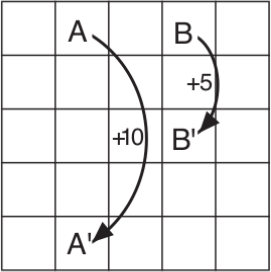
\includegraphics[width = 0.2 \textwidth]{2.21.1.png}
    }
    \hspace{1cm}
    \subfloat[$v_\ast$]
    {
        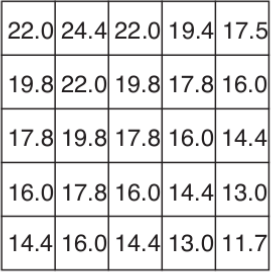
\includegraphics[width = 0.2 \textwidth]{2.21.2.png}
    }
    \hspace{1cm}
    \subfloat[$\pi_\ast$]
    {
        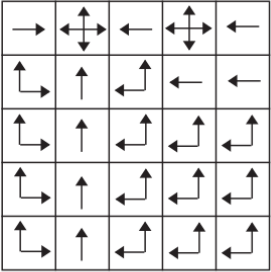
\includegraphics[width = 0.2 \textwidth]{2.21.3.png}
    }
    \hspace{0mm}
    \caption
    {
        Optimal solutions to the gridworld example.
    }
    \label{fig:2.21}
\end{figure}

\end{exercise}

% --------------------------------------------------------------------------------

\begin{solution}

Label the grid positions by $(x, y)$ where $x$ denotes the horizontal and $y$ the vertical position.
$(0, 0)$ should be located at the upper left.

The dynamics of $\pi_\ast$ are simple.
For each position $s$, after a certain number of time steps $t_s$, the player will always fall into the cycle

\begin{align*}
    A \mapsto A^\prime = (1, 0)
      \mapsto (1, 1)
      \mapsto (1, 2)
      \mapsto (1, 3)
      \mapsto (1, 4) = A.
\end{align*}

Note that $t_s$ is actually well defined because no matter what chain of actions (there may be multiple) is taken under $\pi_\ast$, the number of time steps it takes to move from $s$ to $A$ is always the same.
Before falling into that cycle, we collect some reward $r_s$.

\begin{align*}
    v_\ast(s)
    & =
    v_{\pi_\ast}(s) \\
    & =
    \E_{\pi_\ast}[G_t \mid S_t = s] \\
    & =
    \E_{\pi_\ast}
    \bbraces
    {
        \sum_{k=0}^\infty
            \gamma^k R_{t+k+1}
        \mid
        S_t = s
    } \\
    & =
    \sum_{k=0}^\infty
        \gamma^k \E_{\pi_\ast}[R_{t+k+1} \mid S_t = s] \\
    & =
    r_s
    +
    \sum_{k = t_s}^\infty
        \gamma^k \E_{\pi_\ast}[R_{t+k+1} \mid S_t = s] \\
    & =
    r_s
    +
    \sum_{k \in 5 \N + t_s}
        \gamma^k \cdot 10 \\
    & =
    r_s + 10 \sum_{k=0}^\infty \gamma^{5 k + t_s} \\
    & =
    r_s + \frac{10 \gamma^{t_s}}{1 - \gamma^5}
\end{align*}

\begin{verbatim}
    [[21.977 24.419 21.977 19.419 17.477]
     [19.78  21.977 19.78  17.802 16.022]
     [17.802 19.78  17.802 16.022 14.419]
     [16.022 17.802 16.022 14.419 12.977]
     [14.419 16.022 14.419 12.977 11.68 ]]
\end{verbatim}

\end{solution}

% --------------------------------------------------------------------------------


\printbibliography

\end{document}
